\documentclass{article}
\usepackage{pgfplots}
\pgfplotsset{compat=1.18}

\begin{document}

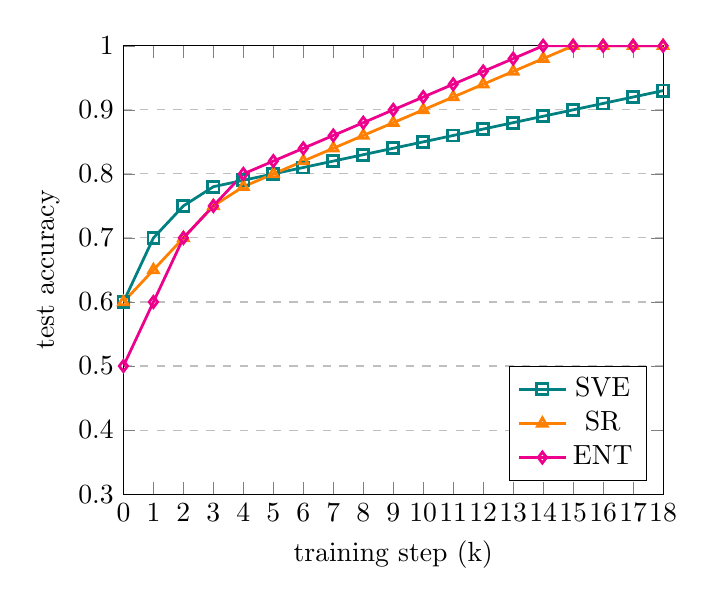
\begin{tikzpicture}
    \begin{axis}[
        xlabel={training step (k)},
        ylabel={test accuracy},
        xmin=0, xmax=18,
        ymin=0.3, ymax=1.0,
        xtick={0,1,...,18},
        ytick={0.3,0.4,...,1.0},
        legend pos=south east,
        ymajorgrids=true,
        grid style=dashed,
    ]
    
    \addplot[
        color=teal,
        mark=square,
        line width=1pt,
    ]
    coordinates {
        (0,0.6)
        (1,0.7)
        (2,0.75)
        (3,0.78)
        (4,0.79)
        (5,0.80)
        (6,0.81)
        (7,0.82)
        (8,0.83)
        (9,0.84)
        (10,0.85)
        (11,0.86)
        (12,0.87)
        (13,0.88)
        (14,0.89)
        (15,0.90)
        (16,0.91)
        (17,0.92)
        (18,0.93)
    };
    \addlegendentry{SVE}
    
    \addplot[
        color=orange,
        mark=triangle,
        line width=1pt,
    ]
    coordinates {
        (0,0.6)
        (1,0.65)
        (2,0.70)
        (3,0.75)
        (4,0.78)
        (5,0.80)
        (6,0.82)
        (7,0.84)
        (8,0.86)
        (9,0.88)
        (10,0.90)
        (11,0.92)
        (12,0.94)
        (13,0.96)
        (14,0.98)
        (15,1.00)
        (16,1.00)
        (17,1.00)
        (18,1.00)
    };
    \addlegendentry{SR}
    
    \addplot[
        color=magenta,
        mark=diamond,
        line width=1pt,
    ]
    coordinates {
        (0,0.5)
        (1,0.6)
        (2,0.7)
        (3,0.75)
        (4,0.80)
        (5,0.82)
        (6,0.84)
        (7,0.86)
        (8,0.88)
        (9,0.90)
        (10,0.92)
        (11,0.94)
        (12,0.96)
        (13,0.98)
        (14,1.00)
        (15,1.00)
        (16,1.00)
        (17,1.00)
        (18,1.00)
    };
    \addlegendentry{ENT}
    
    \end{axis}
\end{tikzpicture}

\end{document}